\newpage

\section{Methodology} \label{methodology}
\subsection{Literature Review} \label{literature_review}
In this chapter, we will describe what literature we have selected, how we have it selected and why we have selected our literature. 
The significance of the literature review lies not only in its ability to contextualize our study within existing scholarship but also in its multifaceted connections to our research questions, chosen methodologies and eventual findings. We followed the upcoming aspects to investigate our research question.
At first we answered the question, whether our work has already been done or not. This is necessary in order to be able to make a statement about how and whether the selected topic is scientifically relevant\footcite[p.34]{adams_research_2014}. There are already a lot of articles about what WebAssemby is, what it may can do or especially a performance comparison between WASM and JavaScript. In the world of software and hardware testing, it has become clear that the smallest differences can change or influence the result. The more tests are carried out, the more results can be compared. Also the more tests you make and the more results you have, the more can be ensured, that the results are valid or not.
In the next step, we pointed out, what the main theoretical perspective is\footcite[p.34]{adams_research_2014}. There are some cases in which WASM is faster than JavaScript and there are also cases, in which JavaScript is faster than WASM. It depends on which explicit test you want to compare JavaScript and WASM\footcite[p.10]{de_macedo_webassembly_2022}. WASM in general promisis a high and optimised performance\footcite{niehoff_webassembly_nodate}. On the other hand, JavaScript is the most common web development language with all its common issues\footcite{mohit_common_nodate}. WASM is build in a binary format, which makes it theoretically faster than Javascript. You can compare these two  on different aspects like Runtime, Memory or cpu usage\footcite[p.1]{sunarto_systematic_2023}. For example, the runtime of WASM is shorter than that of JavaScript in all WasmBoy benchmark tests. There are differences between the various browsers in which the WasmBoy benchmark test was run, with the differences being most noticeable in Mozilla's browser, Firefox\footcite[p.6]{de_macedo_webassembly_2022}. There are also tests in which JavaScript performs better than WASM. In microbenchmark tests in the form of various sorting algorithms, JavaScript sometimes achieves shorter throughput times than WASM. Here too, the results differ depending on the browser used\footcite[p.5]{de_macedo_webassembly_2022}. The memory usage of WASM also differs from JavaScript. WASM uses considerably more memory than JavaScript, both in Firefox and in Chrome. The difference between the memory usage of WASM and JavaScript is increasing as the input given to the two web standards increases. While the memory usage of JavaScript remains the same despite increasing input, the memory usage of WASM increases continuously\footcite[pp.4]{sunarto_systematic_2023}.
After that, we want to show up the problems we got while researching the literature\footcite[p.37]{adams_research_2014}. While gaining general information about the main theoretical perspectives, the problem was, that there was not that single literature which could answer our research question. It was also not easy to find out, how to make our specific tests between these two architectures. There are many different literatures which compared WASM and JavaScript on many different technical aspects but not pointed out, which method may be the best. The topic is also relatively new, which made it difficult to find suitable literature. Both quantitatively and qualitatively.
In the following we will describe the major controversies on our topic\footcite[pp.37]{adams_research_2014}. WASM is not used in common yet. JavaScript is still the most common web development language. One reason for that can be the disadvantage, that a garbage collector is still missed in WASM, which means that storage management can not be done by itself. WASM can also not interact with the DOM of a Website without JavaScript and therefore not change the visualization of a website itself\footcite{bigelow_was_nodate}.

\subsection{Laboratory Experiment} \label{laboratory_experiment}
Platzhalter Text
\subsubsection{Experimental Design} \label{experimental_design}
A scientific experiment is carried out in order to obtain empirical data and to test the hypotheses put forward. To distinguish it from an observation, independent variables are manipulated in an experiment under controlled conditions. The independent variable in turn influences a dependent variable. In the next step, the independent variable is deliberately manipulated and the dependent variable reacts to this event\footcite{genau_experiment_2018}.
For our research, a laboratory experiment comes into question, as we create an artificial environment in which we can control all variables well. Due to the artificial environment we have created, assumptions can be made, but the results cannot be generalized with complete certainty\footcite{genau_experiment_2018}.
In this chapter we describe our experimental design for our explanatory research. 
For our experimental design, we orientated on four key steps that help us to perform a theory based and structured experiment. The four key steps are\footcite{bevans_guide_2019}:
\begin{itemize}
    \item Defining our variables
    \item Writing our hypothesis
    \item Designing our experimental treatments
    \item Measure our dependent variable
\end{itemize}

\newpage

\textbf{Defining our Variables} \newline

\begin{figure}[H]
    \centering
    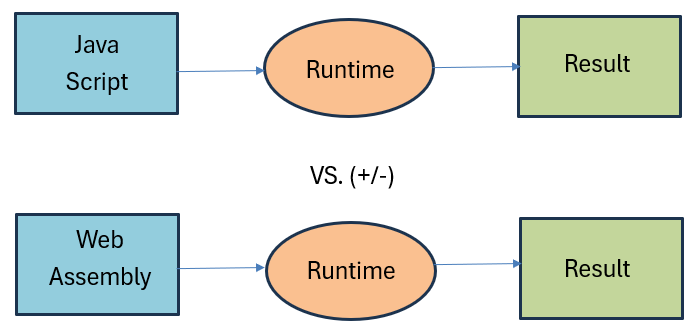
\includegraphics[width=1\textwidth]{Comparison Design.PNG}
    \caption{Comparison Design, Source: Own depiction}
	\label{fig:compdesign}
\end{figure}

In that case our question is, if and how the runtime can be affected by whether using JavaScript or using WASM for different computationally intensive operations. The key independant variables are „JavaScript“ and „WASM“. The key dependant variable is „Runtime“. Abb.X is further called „Fixed testing part“.
To specify different input operations, we will show them in the following figures, while there is the fixed test part as shown above and the "operation part" for the different test operations, which define the input given to each, JavaScript and WASM within the fixed test part.

\begin{figure}[H]
    \centering
    \caption{Advanced Comparison Design, Source: Own depiction}
	\label{fig:comparison}
    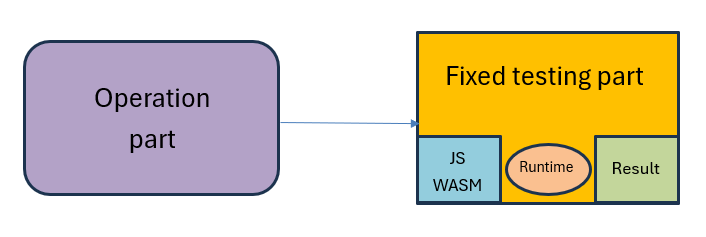
\includegraphics[width=1\textwidth]{Comparison 2.PNG}
\end{figure}

\begin{table}[H]
    \centering
    \caption{Differenciation of dependant and independant variables, Source: Own depiction}
	\label{fig:variables}
    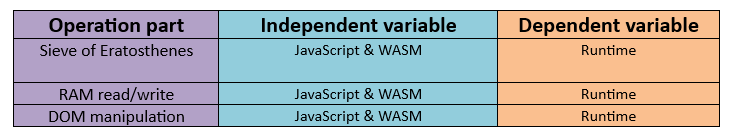
\includegraphics[width=1\textwidth]{Table variables.PNG}
\end{table}

The first operation part is about the Sieve of Eratosthenes. The code is written in both, JavaScript and for WASM with Rust. Both programming languages are the independent variables, which are effecting the dependent variable runtime directly.
The third operation part is about DOM manipulation. Here, the independent variables are JavaScript and WASM. The dependent variable, affected be the independent variables JavaScript and WASM, is runtime.

\textbf{Writing our hypothesis} \newline
Now that we have defined our testing variables, we can put our hypothesis for each operation part in position\footcite{bevans_guide_2019}.

\begin{table}[H]
    \centering
    \caption{Definition of hypothesis for each operation part, Source: Own depiction}
	\label{fig:hypothesis}
    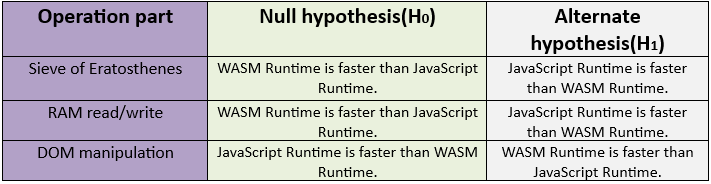
\includegraphics[width=1\textwidth]{Table hypothesis.PNG}
\end{table}

With the execution of the Sieve of Eratosthenes algorithm it is assumed that WASM has a faster Runtime than JavaScript.
For RAM read and write operations it is assumed that WASM has a faster runtime than JavaScript.
For the third hypothesis it is assumed that JavaScript has a faster Runtime than WASM for DOM manipulation.

\textbf{Design our experimental treatments} \newline
In order to carry out a realistic test experiment, it is necessary to make various changes to the variables. This allows a wide variety of conditions to be tested and the resulting findings to be recorded. Different variables ensure that the experiment is as valid as possible\footcite{bevans_guide_2019}.
In our case we simply change the operation part to manipulate our independant variables. By changing this, JavaScript and WASM can be compared on different ways in different use cases, so that we can collect as many results as possible and useful for our comparison and research goal.

\textbf{Measure our dependent variable} \newline
In the end, we will collect all the data from the testing cases (operation part) and measure them, to answer our hypothesis.

\subsubsection{Setup} \label{setup}
In this chapter the experimental setup of this paper and the the corresponding code will be described. Referring to the chapter before, there are three different test that need to be conducted. 

\textbf{Setup Website} \newline
In order to do all tests in one place, a locally hosted website was created. The setup of this website is rather simple yet effective. It consists of a headline and six buttons.
\begin{figure}[H]
    \centering
    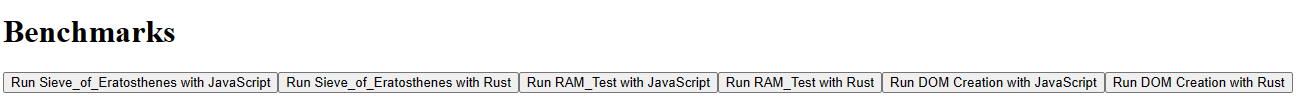
\includegraphics[width=1\textwidth]{website}
    \caption{Benchmark Website, Source: Own depiction}
	\label{fig:website}
\end{figure}

Each button executes one of the tests, three buttons are for the JavaScript tests and the other three for the WASM tests. Before each test is executed, an input window appears and asks the user to enter a number. What the number represents depends on the test that is executed.

The code of the main page of the website looks as follows:
\begin{lstlisting}[language=HTML, caption={HTML Code of the main page of the website, source: self-coded}]
    <!DOCTYPE html>
    <html lang="en">
        <head>
            <meta charset="UTF-8">
            <meta name="viewport" content="width=device-width, initial-scale=1.0">
            <title>Benchmarks</title>
        </head>
        <body>
            <h1>Benchmarks</h1>
            <script type="module" src="./main.JavaScript"></script>
        </body>
    </html>
\end{lstlisting}

This basic HTML Code defines the main structure of the website. In terms of styling, there is none. The main task of this code is to link the main.JavaScript file.  

\textbf{Setup First Test - CPU Benchmark} \newline
Next is the setup of the first test, which is a CPU Benchmark test based on the Sieve of Eratosthenes algorithm. In the field of computer science this algorithm is commonly used to measure computer performance. "The time complexity of calculating all primes below n in the random access machine model is \( O(n \log \log n) \) operations, a direct consequence of the fact that the prime harmonic series asymptotically approaches \( \log \log n\). It has an exponential time complexity with regard to input size, though, which makes it a pseudo-polynomial algorithm. The basic algorithm requires \( O(n) \) of memory."\footcite{wikipedia_sieve_2024}.
The input parameter for this test determines the limit up to where the algorithm searches for prime numbers.

The following code was used to execute the algorithm with JavaScript:
\begin{lstlisting}[language=JavaScript, caption={Sieve of Eratosthenes in JavaScript, source: self-coded}]
function JavaScript_sieve(limit) {
    // Create an array to track whether each number is prime
    const sieve = new Array(Number(limit) + 1).fill(true);
    // 0 and 1 are not prime numbers, so mark them as false
    sieve[0] = sieve[1] = false;
    // Initialize an empty array to store prime numbers
    const primes = [];
    // Iterate through the numbers starting from 2 up to the square root of the limit
    for (let i = 2; i <= Math.sqrt(limit); i++) {
        // If the current number is prime (marked as true), proceed
        if (sieve[i]) {
            // Mark multiples of the current prime number as not prime
            // Starting from i*i, as all numbers below that would have been already marked
            for (let j = i ** 2; j <= limit; j += i) {
                sieve[j] = false;
            }
        }
    }
    // Iterate through the sieve to extract prime numbers
    for (let i = 0; i < sieve.length; i++) {
        if (sieve[i]) {
            primes.push(i);
        }
    }
    // Return the array of prime numbers
    return primes;
}
\end{lstlisting}

The following code was used to execute the algorithm with WASM, coded in Rust:
\begin{lstlisting}[language=Rust, caption={Sieve of Eratosthenes in Rust, source: self-coded}]
#[wasm_bindgen]
pub fn wasm_sieve(limit: usize) -> Vec<usize> {
    // Create a boolean vector to track whether each number is prime
    let mut sieve: Vec<bool> = vec![true; limit + 1];
    let mut primes: Vec<usize> = Vec::new();
    // 0 and 1 are not prime numbers, so mark them as false
    sieve[0] = false;
    sieve[1] = false;
    // Iterate through the numbers starting from 2 up to the square root of the limit
    for i in 2..=(limit as f64).sqrt() as usize {
        // If the current number is prime (marked as true), proceed
        if sieve[i] {
            // Mark multiples of the current prime number as not prime
            // Starting from i*i, as all numbers below that would have been already marked
            for j in (i * i..=limit).step_by(i) {
                sieve[j] = false;
            }
        }
    }
    // Iterate through the sieve to extract prime numbers
    for i in 2..=limit {
        if sieve[i] {
            primes.push(i);
        }
    }
    // Return the vector of prime numbers
    primes
}
\end{lstlisting}

Both code snippets in essence implement the same algorithm, just in different languages. However, it was coded in such a way that the implementations are comparable. To give an example, the code written in Rust could be further optimized by iterating over the sieve vector with `sieve.iter()`. Since this is not an option in JavaScript it was implemented similarly to JavaScript to enhance comparability. Another difference between both implementations is the usage of vectors in Rust. Because the neither the input nor the number of primes is not known beforehand, a growable object is required. In JavaScript an array is such a growable object but in Rust an array is not growable, therefore it is replaced by a vector. 

\textbf{Setup Second Test - RAM Speed} \newline
The second test uses a multitude of read and write operations as a stress test for the RAM speed. The input parameter for this test determines the size of the iterable to perform the read and write operations on.

The following code was used to execute the stresstest with JavaScript:
\begin{lstlisting}[language=JavaScript, caption={RAM stresstest in JavaScript, source: self-coded}]
function JavaScript_ram_test(size) {
    const array = new Array(size);
    // Write operation
    for (let i = 0; i < size; i++) {
        array[i] = i;
    }
    // Read operation
    for (let i = 0; i < size; i++) {
        array[i] += 1;
    }
}
\end{lstlisting}

The following code was used to execute the stresstest with WASM, coded in Rust:
\begin{lstlisting}[language=Rust, caption={RAM stresstest in Rust, source: self-coded}]
#[wasm_bindgen]
pub fn wasm_ram_test(size: usize) {
    let mut vec: Vec<usize>  = Vec::with_capacity(size);
    // Write operation
    for i in 0..size {
        vec.push(i);
    }
    // Read operation
    for i in 0..size {
        vec[i] += 1;
    }
}
\end{lstlisting}

As with the first test, the two code snippets, in essence, execute the same operations. The difference in both implementations are identical to the previous test and are also justified the same way. 

\textbf{Setup Second Test - DOM manipulation} \newline
The final test was about DOM manipulation and was implemented because JavaScript "makes it relatively easy to manipulate the DOM (i.e., add, modify, and remove elements), but does nothing to promote doing so efficiently"\footcite{peterson_10_nodate}. Therefore this test investigates the DOM manipulation with JavaScript and WASM to see which operates more efficiently. The input parameter for this test determines the number of div elements that should be created and shown on the screen.

The following code was used to execute the DOM manipulations with JavaScript:
\begin{lstlisting}[language=JavaScript, caption={DOM manipulation in JavaScript, source: self-coded}]
function JavaScript_create_elements(count) {
    // Get a reference to the document body
    const body = document.body;
    // Iterate 'count' times to create elements
    for (let i = 0; i < count; i++) {
        // Create a new div element
        const div = document.createElement("div");
        // Set styles for the div element
        div.style.border = "2px solid #000";
        div.style.backgroundColor = "#e0e0e0";
        div.style.margin = "5px";
        // Set text content for the div element
        div.textContent = "Hello, JavaScript!";
        // Append the div element to the document body
        body.appendChild(div);
    }
}
\end{lstlisting}

The following code was used to execute the algorithm with WASM, coded in Rust:
\begin{lstlisting}[language=Rust, caption={DOM manipulation in Rust, source: self-coded}]
#[wasm_bindgen]
pub fn wasm_create_elements(count: usize) {
    // Access the document object from the web_sys crate
    let document = web_sys::window().unwrap().document().unwrap();
    // Iterate 'count' times to create elements
    for _ in 0..count {
        // Create a new div element
        let div = document.create_element("div").unwrap();
        // Set styles for the div element
        div.set_attribute("style", "border: 2px solid #000; background-color: #e0e0e0; margin: 5px;").unwrap();
        // Set text content for the div element
        div.set_text_content(Some("Hello, WASM!"));
        // Append the div element to the document body
        document.body().unwrap().append_child(&div).unwrap();
    }
}
\end{lstlisting}

In this case the two code snippet again implement the same procedure. Unlike in the previous tests, there are no performance-relevant differences between JavaScript and WASM. The difference in the code emerge from the syntax of the two languages. However, one difference needs to be highlighted. Rust encourages explicit error handling. Since this code will not be deployed to regular users, explicit error handling is not necessary and is avoided by using the `.unwrap()` function.

One aspect of all Rust-specific tests is the \texttt{\#[wasm\_bindgen]} command before every function which is described by mdn web docks as follows "wasm-pack uses wasm-bindgen, another tool, to provide a bridge between the types of JavaScript and Rust. It allows JavaScript to call a Rust API with a string, or a Rust function to catch a JavaScript exception"\footcite{mozilla_compiling_nodate}. This command is essential for the main.JavaScript to access the Rust functions when a test is triggered, therefore it is another important of this chapter. 
\subsubsection{Procedure} \label{procedure}
The structure of each test case was identical. The respective test is started via a button, which opens a pop-up window in which the input for the test is entered. The input is then confirmed and the following code is executed:
\begin{verbatim}
document.addEventListener("DOMContentLoaded", function () {
    init();
    console.log("Loaded");
    for (const [testName, testFunctions] of Object.entries(funcs)) {
        for (const [index, implementation] of testFunctions.entries()) {
            const button = document.createElement("button");
            button.textContent = `Run ${testName} with ${rust_JavaScript[index]}`;
            button.addEventListener("click", () => {
                const input = prompt("Input:");
                let totalTime = [];
                let output;
                for (let i = 0; i < runs; i++) {
                    const startTime = performance.now();
                    output = implementation(input);
                    const endTime = performance.now();
                    console.log(output);
                    const elapsedTime = endTime - startTime;
                    totalTime.push(elapsedTime);
                    console.log(`Run ${i + 1}: ${elapsedTime} milliseconds`);
                }
                const averageTime = totalTime.reduce((a,b) => a+b, 0) / runs;
                console.log('Total time:', totalTime)
                console.log(`Function ${testName}, ${rust_JavaScript[index]} with input ${input} took ${averageTime} miliseconds to execute`);
            });
            document.body.appendChild(button);
        }
    }
});
\end{verbatim}
caption einfügen

In order to allow a structured testing procedure, the tests were executed in the following order:
\begin{enumerate}
\item The first test was started with an input of 100.000.000 and was repeated 10 times for JavaScript and 10 times for WASM.
\item The second test was started with an input of 100.000.000 and was repeated 10 times for JavaScript and 10 times for WASM.
\item We started the third test with an input of 30.000 and ran it five times each for JavaScript and for WASM.
\end{enumerate}
The result of each test is output via the command line and then recorded in a table. The table will be presented later on in the chapter results.

In addition, the average runtime, standard deviation and factor by which WASM is executed faster or slower than JavaScript, relative to the average runtime, was calculated and added to the table.
\subsection{Research Project} \label{research_project}
    The paper focuses on WASM. However, as Business Informatics students, we also aimed to explore professional collaboration in academic paper writing. We embraced the challenge of writing the paper using LaTeX, which required learning LaTeX syntax, setting up and structuring a LaTeX project, and understanding LaTeX source management.

    Furthermore, the paper was collaboratively developed among the three researchers. We created a GitHub repository for the entire LaTeX project, just like for the experiment's code. This decision provided valuable insights and learnings which is important for our academic future since it is common practice in technical scientific papers to use LaTeX with a Git version control (!Quelle: actuarial, medium).

    A consequence of these decisions was our agreement to work collectively in Microsoft Visual Studio Code using the 'LaTeX Workshop' plugin by James Yu, ensuring uniform technical capabilities among us. We considered an alternative, which was using Overleaf, an online LaTeX editor. However, this would have created costs for collaborative work, which we chose to avoid.

    Subsequent chapters of this paper provide a more detailed analysis of LaTeX and GitHub, highlighting the challenges encountered during the process.
\subsubsection{Latex Project} \label{latex_project}
As mentioned earlier, we wanted to challenge ourselves by writing this paper in \LaTeX{}. \LaTeX{} is based on the markup language TeX, originally developed by the American computer scientist Donald Knuth in 1982. The \LaTeX{} framework used for this project is "a macro package built on top of TeX", intended to "simplify the typesetting of TeX" (!source: Wikibooks). Essentially, a \LaTeX{} document is nothing more than a text document enriched with commands and markup.

One of the main differences between \LaTeX{} and conventional text editors such as Microsoft Word is that the author does not immediately see the result of what he is writing. Unlike MS Word, which operates on the principle of WYSIWYG (What You See Is What You Get), \LaTeX{} operates on the principle of WYSIWYAF (What You See Is What You Asked For).

Despite the significant drawback of requiring authors to learn how to use \LaTeX{}, the advantages outweigh the disadvantages. Wikibooks outlines the advantages of \LaTeX{} as follows:

- You can concentrate purely on the structure and contents of the document. \LaTeX{} will automatically ensure that the typography of your document—fonts, text sizes, line heights, and other layout considerations—are consistent according to the rules you set.
- In \LaTeX{}, the document structure is visible to the user, and can be easily copied to another document. In WYSIWYG applications it is often not obvious how a certain formatting was produced, and it might be impossible to copy it directly for use in another document.
- Indexes, footnotes, citations and references are generated easily and automatically.
- Mathematical formulae can be easily typeset. (Quality mathematics was one of the original motivations of TeX.)
- Since the document source is plain text,
    - Document sources can be read and understood with any text editor, unlike the complex binary and XML formats used with WYSIWYG programs.
    - Tables, figures, equations, etc. can be generated programmatically with any language.
    - Changes can be easily tracked with version control software.
- Some academic journals only accept or strongly recommend submissions in the form of \LaTeX{} documents. Publishers offer \LaTeX{} templates.
(!Source: Wikibooks).

We found these points to be significant advantages in our work with \LaTeX{}, particularly the highly structured approach to document composition and the straightforward handling of sources.

However, a simple \LaTeX{} document would not suffice. The most effective use of \LaTeX{} is to set up an entire \LaTeX{} project, especially when different sections of the paper are written simultaneously by different contributors. Such a \LaTeX{} project allows each part of the structure of the paper, such as chapters including all subchapters, to be divided into individual files. These individual files can then be worked on independently, as they are simply referenced within the existing structure (in our case, from a parent chapter file). This provides the flexibility to create the structure of the whole document without content, and then modify the structure without having to consider the content layout. Furthermore, as mentioned in the advantages of Wikibooks, it is possible to change aspects such as layout and font size centrally.

That is why we decided to take on the challenge of writing this paper in \LaTeX{}. Now we will go into the detailed structure of our \LaTeX{} project.

Fortunately, we were able to adopt the general structure from Andy Grunwald, a former FOM student, who has published a "FOM \LaTeX{} template" on GitHub (!Source: GitHub Repository). This template has many contributors and is continuously improved and adapted to FOM-specific requirements.

In addition to providing the basic document structure, the template also provides various methods for compiling the associated PDF document for the project. This includes using the provided docker file or the compilation files together with the VS Code extension "\LaTeX{} Workshop" by James Yu.

Now let's look at the basic structure of the \LaTeX{} document itself. There is a main file called "thesis_main.tex" which describes the basic configurations for the document, such as font size, font, margins, etc., and defines the structural layout of the thesis. This is done using the `\input{}` method, where the path to the referenced file is enclosed in curly braces. This provides a concise and easy to understand method of defining the structure.

The content chapters are further encapsulated, each having its own "structure file" (e.g. chapterOverview.tex). This file references individual chapters, each of which can have its own respective structure. Here is an overview of the structure of the document:

(!Darstellung einfügen)

This ensures that the substantive parts (the chapters and subchapters) are separated from the more administrative parts, such as the table of contents. This clear separation is particularly helpful in academic papers where the style, such as numbering, may vary from section to section. With this clear separation, it is possible to apply different styles to each section.

Certainly, other methods would be sufficient for a term project and would achieve similar or identical results. However, as mentioned earlier, we wanted to overcome this technical challenge so that we could use it for future projects.
\subsubsection{Github} \label{github}
GitHub is a web-based version control system for software development that allows developers to manage their code in private or public repositories. Although there are many alternatives, such as GitLab, Bitbucket or SourceForge, we chose GitHub mainly because of its seamless integration with Microsoft Visual Studio Code, the chosen editor for this project.

The benefits of a centralised version control are obvious. On the one hand, it allows the entire project to be managed in one place, ensuring that it is always the latest version. On the other hand, a GitHub repository, even if set to private, facilitates collaborative and platform-independent work on the project.

In theory, GitHub's ability to create project and organisational structures could make it much easier to scale up research projects. In addition to managing such projects through Git pull and push requests, GitHub offers effective use of built-in features such as issues and discussions to challenge others' contributions, leading to the development of better and more refined ideas.

However, to maintain the focus and scope of this paper, we have chosen to use GitHub exclusively as a version control system. There is a repository called \dq WASMvsJavaScript\dq  for the development of the experiment (!Quelle GitHub Repo), and another called \dq ITInfraPaper\dq  for the \LaTeX{} project (!Quelle GitHub Repo). Both repositories are publicly accessible and linked in the source directory.


% -----------------------------------
% Teil aus der Vorlage
% -----------------------------------

% \section{Latex-Details} \label{latexDetails}

% \subsection{Verwendete Software, Editor und Zusatzpakete}
% \subsubsection{Windows 8+}
% \begin{itemize}
% \item MikTex: 2.9, 32-bit
% \item Biblatex: 3.5, Zusatz: Biber.exe
% \item Editor: TexStudio (kann ich empfehlen), Notepad++
% \end{itemize}

% \subsubsection{Mac OSX und iOS}
% \begin{itemize}
% \item MacTeX: \url{https://tug.org/mactex}
% \item Editor: TexPad \url{https://www.texpadapp.com}
% \end{itemize}

% \subsubsection{Online}
% Overleaf ist eine Online-Anwendung mit der Ihr direkt im Browser an eurer Thesis schreiben könnt. Bis 1GB Größe und maximal 60 Einzeldateien könnt ihr Overleaf kostenlos nutzen: \url{https://www.overleaf.com/}


% \subsection{Dokumentenklasse}
% Eigentlich hatte Prof. Finke empfohlen die Dokumentklassen \enquote{Book} oder \enquote{Report} für die Erstellung der Bachelor-Thesis zu verwenden, da diese über weitere Gliederungsebenen verfügen. Ich verwende dennoch eine leicht modifizierte Komaskript-Klasse \enquote{scrartcl}, mit der Erweiterung um eine Ebene. Siehe (skripte/weitereEbene.tex). Das Skript stammt irgendwo aus den Netz und übersteigt meine \LaTeX{}-Fähigkeiten. Dadurch kann ich über eine weitere Ebene in der Arbeit verfügen, ohne mich mit der Modifikation von chapter-Seiten rumschlagen~\footcite[Vgl. ][S. 5]{Tanenbaum.2003} zu müssen. Diese Quelle ist nur zur Demonstration und hat keinen inhaltlichen Bezug hierzu. Es werden übrigens nur die Quellen im Literaturverzeichnis angezeigt, die auch referenziert sind.


% \subsection{Grafiken}
% Das Paket \textbackslash usepackage\{float\} ermöglicht es die Grafiken und Tabellen an der Stelle im Text zu positionieren, wo diese im Quelltext stehen (Option H). Ansonsten würde \LaTeX{} diese dort unterbringen, wo es typographisch sinnvoll wäre - das wollen wir ja nicht ;-).

% Die Breite der Grafiken am Besten relativ zum Text angeben.

% \subsection{Quellcode}
% Quellcode kann auf unterschiedliche Arten eingebaut werden.
% Zum einen kann es hier durch direktives Einbinden in der chapter-Datei geschehen.
% \begin{lstlisting}
% Hier wird aufgezeigt, wie man eine Grafik einbindet, es wird also in der PDF angezeigt,
% da es in einem Quellcode-Listing steht.
% Auch wenn es hier faelschlicherweise als LaTeX-Befehl angezeigt wird.
% 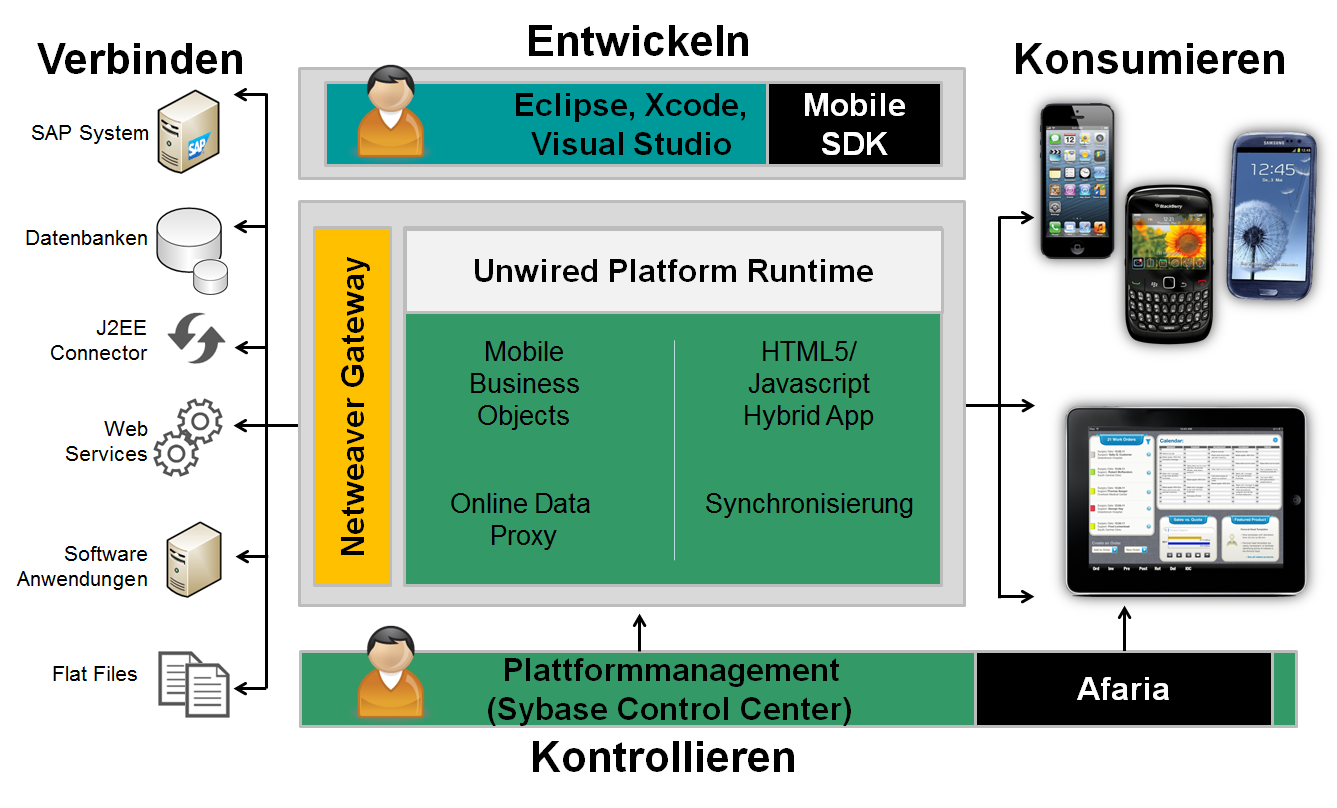
\includegraphics[width=0.9\textwidth]{sup}
% \end{lstlisting}

% Bei längeren Quellcode-Listings empfiehlt es sich jedoch auf eine externe Datei im Ordner Quellcode zu verlinken und diese einzubauen:
% \lstinputlisting[language=HTML]{./Quellcode/Beispiel.html}

% Statt dem Package lstlisting, welches direkt auf Tex basiert, kann auch das Package minted verwendet werden.
% Dieses Package basiert auf python-pygments und unterstützt weit mehr Sprachkonstrukte als lstlisting.
% Um das Paket zu verwenden muss es eingebunden werden und zusätzlich python-pygments installiert sein.
% (Dies ist mit im Dockerfile vorhanden. Für die anderen Compile-Methoden, wie das native verwenden von Tex Live findet sich hier die Installationsanleitung für das minted Paket: https://ctan.org/pkg/minted?lang=de)

% Damit das kompilieren ohne Python trotzdem möglich ist, ist die Funktion standardmäßig ausgebaut. Deshalb muss zusätzlich in der Datei \begin{verbatim}thesis_main.tex \usepackage{minted} \end{verbatim} wieder einkommentiert werden. 

% Minted lässt sich dann ganz ähnlich zu lstlisting verwenden:
% \begin{lstlisting}
% 	\begin{minted}{c}
% 		int main() {
% 			printf("hello, world");
% 			return 0;
% 		}
% 	\end{minted}
% \end{lstlisting}	

% Da der Pfad zu den Abbildungen im Hauptdokument definiert wurde, muss hier nur noch der Name des Bildes ohne Dateiendung stehen (sup).

% \begin{figure}[H]
% \caption{Titel der Abbildung hier}
% 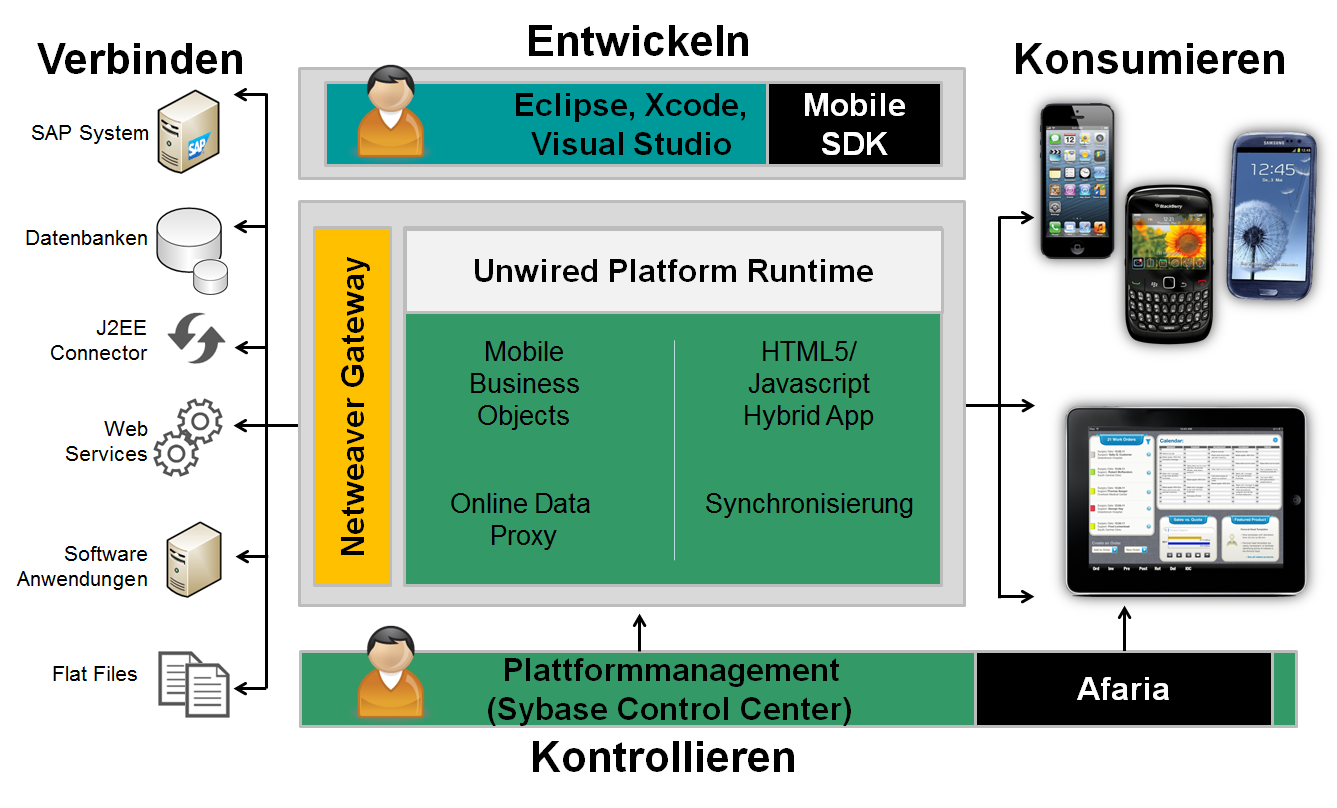
\includegraphics[width=0.9\textwidth]{sup}
% \\
% Quelle: Eigene Darstellung
% \end{figure}

% \subsection{Tabellen}
% \begin{table}[H]
% \caption{Beispieltabelle 1}
% \label{tbl:beispieltabelle2}
% \begin{tabularx}{\textwidth}[ht]{|l|X|l|}
%   \hline
%   \textbf{Abkürzung} & \textbf{Beschreibung} & \textbf{Berechnung}\\
%   \hline\hline
%     MEK & Materialeinzelkosten & \\
%   	MGK & Materialgemeinkosten & $+ \uparrow$~*\\
%     FEK & Fertigungseinzelkosten & \\
%   	FGK & Fertigungsgemeinkosten & $+ \uparrow$~*\\
% 	SEKF & Sondereinzelkosten der Fertigung & \\
% 	\hline\hline
% 	\multicolumn{3}{|l|}{\textbf{= Herstellungskosten}} \\
% 	\hline\hline
%   	VwGK & Verwaltungsgemeinkosten & $+ \uparrow$~*\\
%   	VtGK & Vertriebsgemeinkosten & $+ \uparrow$~*\\
%   	SEKVt & Sondereinzelkosten des Vertriebes & \\
% 	\hline\hline
% 	\multicolumn{3}{|l|}{\textbf{= Selbstkosten}} \\
% 	\hline\hline
% 	\multicolumn{3}{|l|}{+ Gewinnaufschlag} \\
% 	\multicolumn{3}{|l|}{+ Rabatte} \\
% 	\hline\hline
% 	\multicolumn{3}{|l|}{\textbf{= Nettoverkaufspreis (NVP)}} \\
% 	\hline
% 	\multicolumn{3}{|l|}{+ Umsatzsteuer} \\
% 	\hline\hline
% 	\multicolumn{3}{|l|}{\textbf{= Bruttoverkaufspreis (BVP)}} \\
% 	\hline
% \end{tabularx} \\
% \cite[Quelle: In Anlehnung an][S. 4]{Beckert.2012}
% \end{table}

% \clearpage % hiermit werden alle Bilder Tabellen ausgeworfen

% \subsection{Biblatex}
% \subsubsection{Erklärung}
% Von den vielen verfügbaren Literatur-Paketen habe ich mich für Biblatex entschieden. Die Anforderungen der FOM sollten hiermit erfüllt sein. Ich habe bisher nur Einträge \enquote{@book} getestet. Wie immer steckt der Teufel hier im Detail und es wird sich später herausstellen, ob Biblatex eine gute Wahl war. Die Anpassungen hierfür liegen unter skripte/modsBiblatex. Ich verwende das Backend Biber, welches bib-Dateien in UTF-8 verarbeiten kann.

% In der für den Leitfaden 2018 aktualisierten Version sind außerdem Beispiele für \enquote{online},\footcite[Vgl.][]{website:angular:aboutAngular} also Webseiten, und \enquote{article},\footcite[Vgl.][S. 140]{Decker2009} also wissenschaftliche Artikel, enthalten.

% Laut Leitfaden sollen maximal 3 Autoren genannt werden und danach mit
% \enquote{et. al.} bzw. \enquote{u.a.} ergänzt werden. Damit im Literaturverzeichnis auch nur max.
% 3 Autoren stehen, muss man beim Füllen der literatur.bib-Datei darauf achten auch nur 3
% einzutragen. Weitere Autoren kann man einfach mit \enquote{and others} ergänzen.
% Siehe Eintrag für \enquote{Balzert.2008}. Zitiert man dann diese Werk, werden auch in
% der Fussnote alle Autoren korrekt genannt wie in dieser
% Fußnote\footcite[Vgl.][S. 1]{Balzert.2008} zu sehen ist.

% Hat man dagegen mehr als 3 Autoren in der bib-Datei hinterlegt, stehen im
% Literaturverzeichnis alle drin. In der Fussnote dagegen, steht nur
% einer\footcite[Vgl.][S. 1]{Balzert2.2008}, was dem Leitfaden widerspricht.

% Die Anzahl von 3 wird übrigens über die Option \enquote{maxcitenames=3} des
% biblatex-Packages gesetzt. Man muss selbst schauen, dass die Anzahl der Autoren
% in den Bib-Dateien mit der Optionseinstellung übereinstimmt.

% \subsubsection{Beispielfußnoten}
% Diese Fussnote soll zeigen, wie mit einem \enquote{von} vor dem Namen des Autors
% umgegangen wird\footcite[Vgl.][S. 1]{Lucke2018}. Man muss für die korrekte
% Sortierung eines solchens Namens im Literaturverzeichnis einen \enquote{sortkey}
% setzen.

% Diese Fussnote soll zeigen, wie mit einer Online-Quelle ohne Jahresangabe
% umgegangen wird\footcite[Vgl.][]{Belastingdienst}.

% Diese Fußnote\footcite[Vgl.][S.1]{Beckert.2012} ist nur dazu da zu zeigen, wie mit mehreren Quellen des selben Autors aus dem selben Jahr umgegangen wird, wenn das Stichwort gleich bleibt \footcite[Vgl.][S.2]{Beckert.2012.1} oder sich ändert\footcite[Vgl.][S.3]{Beckert.2012.2}. Laut Leitfaden sollte bei gleichem Autor, Jahr und Stichwort ein Buchstabe an die Jahreszahl gehangen werden. Zum Beispiel 2012a. 

% Die folgenden Fußnoten dienen dazu zu zeigen, dass die Nummern von zwei direkt aufeinanderfolgende Fußnoten mit Komma getrennt werden.\footcite[Vgl.][S.2]{Beckert.2012.1}\footcite[Vgl.][S. 1]{Lucke2018}
% \subsection{Abkürzungen}
% Abkürzungen werden mithilfe des Pakets Acronym eingebunden. Alle Abkürzungen sollten in der Datei acronyms.tex mithilfe des \begin{verbatim}
% 	\acro
% \end{verbatim} Befehls festgelegt werden. Im Text werden diese dann mit \begin{verbatim}
% 	\ac{Abkürzung}
% \end{verbatim} benutzt. Bei der ersten Verwendung einer Abkürzung wird der Begriff in beiden Formen dargestellt. So wie hier: \ac{WYSIWYG}. Nur wenn eine Abkürzung tatsächlich verwendet wird erscheint sie auch im Abkürzungsverzeichnis.

% Sollte es im Abkürzungsverzeichnis zu Anzeigefehlern kommen kann dies daher rühren, dass eine Abkürzung verwendet wird, die länger ist als \ac{WYSIWYG}. In diesem Fall müsst ihr in der Datei acronyms.tex den Parameter [WYSIWYG] durch eure längere Abkürzung ersetzen.

% \subsection{Formeln}
% Um eine Formel nach links aus zurichten muss sie zwischen \& und \& eingesetzt werden:

% \textbf{Formel 1: Erste Formel}
% \begin{flalign}
%    & L_P{=} 10lg \cdot \frac{P}{1 mW} &
% \end{flalign}
% \cite[Quelle: In Anlehnung an][S. 4]{Beckert.2012}


% Etwas mehr Text.

% Ansonsten wird sie mittig ausgerichtet test.
% Mehr infos: http://www.ctex.org/documents/packages/math/amsldoc.pdf

% \textbf{Formel 2: Zweite Formel}
% \begin{flalign}
%    L_P{=} 10lg \cdot \frac{P}{1 mW}
% \end{flalign}
% \cite[Quelle: In Anlehnung an][S. 4]{Beckert.2012}

% \subsection{Symbole}
% die folgenden Symbole haben nicht mit der Formel oben drüber zu tun
% Das hier ist ein definiertes Symbol: \symnz und das hier auch \AB . Symbole werden in der Datei Skripte symboldef.tex zentral definiert.

% \subsection{Glossar}
% Begriffserklärungen bzw. das \gls{glossar} wird mithilfe des Pakets \gls{glossaries} eingebunden. Alle Begriffe die erklärt werden sollen, sollten in der Datei glossar.tex mithilfe des \begin{verbatim}
% 	\newglossaryentry
% \end{verbatim} Befehls festgelegt werden. Im Text werden diese dann mit \begin{verbatim}
% 	\gls{Begriff}
% \end{verbatim} benutzt.


% \subsection{Listen und Aufzählungen}
% \subsubsection{Listen}
% \begin{itemize}
% \item ein wichtiger Punkt
% \item noch ein wichtiger Punkt
% \item und so weiter
% \end{itemize}
% \subsubsection{Aufzählungen}
% \begin{enumerate}
% \item Reihenfolge ist hier wichtig
% \item Dieser Punkt kommt nach dem ersten
% \item Da sollte jetzt eine 3 vorne stehen
% \end{enumerate}

% \paragraph{Tiefste Ebene 1}
% Dies ist die tiefste Gliederungsebene. Sollten doch mehr Ebenen benötigt werden, muss eine andere Dokumentenklasse verwendet werden.

% \paragraph{Tiefste Ebene 2}
% Der zweite Punkt in dieser Ebene ist zur Erinnerung daran, dass es nie nie niemals nur einen Unterpunkt geben darf.

% \subsection{Skript zum Kompilieren}
% Latex will ja bekanntlich in einer bestimmten Reihenfolge aufgerufen werden:
% \begin{lstlisting}
% lualatex thesis_main.tex
% biber thesis_main
% lualatex thesis_main.tex
% lualatex thesis_main.tex
% thesis_main.pdf
% \end{lstlisting}

% Dies ist der Inhalt der Batchdatei \enquote{compile.bat}.

% \subsection{PlantUML}

% \begin{lstlisting}
% \begin{plantuml}
% @startuml
% Class01 <|-- Class02
% Class03 *-- Class04
% Class05 o-- Class06
% Class07 .. Class08
% Class09 -- Class10
% @enduml
% \end{plantuml}
% \end{lstlisting}
